\chapter{Experiments}
\label{chapter:ch4}

In this chapter the process and results of multiple experiments, that look into performance of various pre-trained feature extractors in industrial anomaly detection tasks, will be presented. First experiment serves to determine the layers of vision transformer architecture that would provide the highest accuracy for anomaly detection when applied as backbones. Secondly, we will provide a performance comparison between different types of deep learning visual models as feature extractors on the PatchCore model, in order to determine which architecture should be chosen for further experiments. Next, the analysis on the efficacy of self-supervised model DINO against supervised classification task training, helping us to make the decision for verifying the method for feature learning. Further, we test the feature space learned from the dataset constructed by the method of selective extraction using CNN bi-class classifiers. Generated feature space competes against one of the state-of-the-art feature spaces for industrial anomaly detection: WideResNet50. Lastly, we will engage in a comparative analysis of the efficiency of the feature space based on a dataset extracted through a method that employs both large language models (LLMs) and visual language models (VLMs). Through these comprehensive experiments and analyses, we aim to derive valuable insights and optimal approaches for advancing industrial anomaly detection by approaching the task as a feature space problem.

\section{Scoring methodology}

\subsection{Scoring metric}
For all the experiments, in order to measure the accuracy of the models being tested, we use AUROC (Area Under the Receiver Operating Characteristic curve) metric. AUROC metric represent the models capability to determine true positives while keeping the number of false positives relatively low. ROC curve, as shown in the figure \ref{fig:auroc}, is the curve that represents the relationship between TPR and FPR at any given threshold. TPR and FPR at an arbitrary threshold is calculated by equations \ref{eq:tpr} and \ref{eq:fpr} respectively. AUROC score is represented as a number between 0 and 1.0(higher the better) and generally, the score 0.5 represents the random guessing. Therefore, scores below 0.5 are considered worse than random guessing while above 0.5 are better. Figures in this paper represent the AUROC score as the percentage from 0\% to 100\%.

\begin{equation}
	TPR = \frac{\text{True Positives}}{\text{True Positives} + \text{False Negatives}}
	\label{eq:tpr}
\end{equation}

\begin{equation}
	FPR = \frac{\text{False Positives}}{\text{False Positives} + \text{True Negatives}}
	\label{eq:fpr}
\end{equation}

\begin{figure}[h]
	\begin{center}
		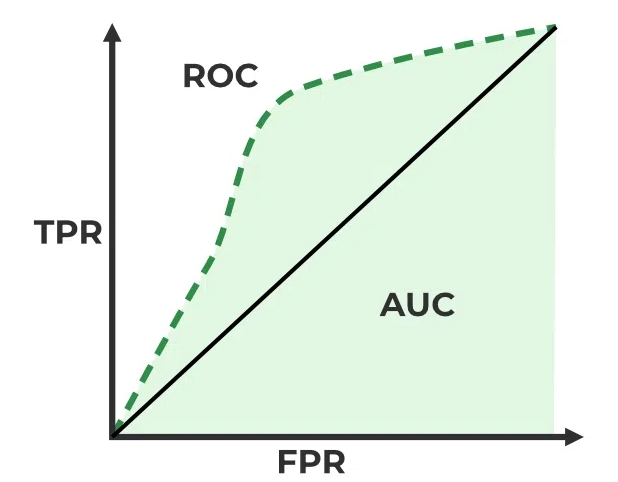
\includegraphics[width=0.5\linewidth]{Chapter_4/auroc.png}
	\end{center}
	\caption{Medical Visual Question Answering (VQA) \cite{liu2021slake} is a task where the model receives medical images and corresponding questions as input and produces accurate answers as the output.}
	\label{fig:auroc}
\end{figure}

\subsection{Industrial Anomaly detection model}
The model of choice for all the tests is the PatchCore model, as it allows an easy plug and play approach to pre-trained feature extractors. PatchCore outputs three types of scores for each category in the MVTechAd dataset. There are also mean scores over all cotegories provide for each type of scores. Types of scores are as follows:

\begin{description}
  \item[Instance AUROC] represents AUROC score for classifying each image as anomalous or nominal
  \item[Anomaly Pixel AUROC] represents AUROC score for classifying each pixel as anomalous or nominal, calculated only on images that contain anomalies
  \item[Full Pixel AUROC] represents AUROC score for classifying each pixel as anomalous or nominal, calculated over all images
\end{description}

In order to be able to utilize Vision Transformer architectures with PatchCore model, the following changes have been made. These changes detect if the ViT is being used as pre-trained feature extractor and reshape the layers as appropriate for PatchCore.

\lstset{frame=tb,
  language=Python,
  aboveskip=3mm,
  belowskip=3mm,
  showstringspaces=false,
  columns=flexible,
  basicstyle={\small\ttfamily},
  numbers=none,
  numberstyle=\tiny\color{gray},
  breaklines=true,
  breakatwhitespace=true,
  tabsize=3
}
\begin{lstlisting}
def patchify(self, features, return_spatial_info=False):
	#...
	if len(features.shape) == 3:
		features = features.transpose(1, 2)
		if features.shape[2] == 197:
			features = features[:, :, 1:]
		hw = int(math.sqrt(features.shape[2]))
		features = features.view(features.shape[0], features.shape[1], hw, hw)
	#...
\end{lstlisting}

\section{Comparison of ViT layers}
\label{vit layers}

In the first experiment we will be analysing the difference of the layers of vision transformer architectures. Throughout the experiment we use VitB/16 pre-trained on ImageNet classification task. 

\begin{figure}[h]
	\begin{center}
		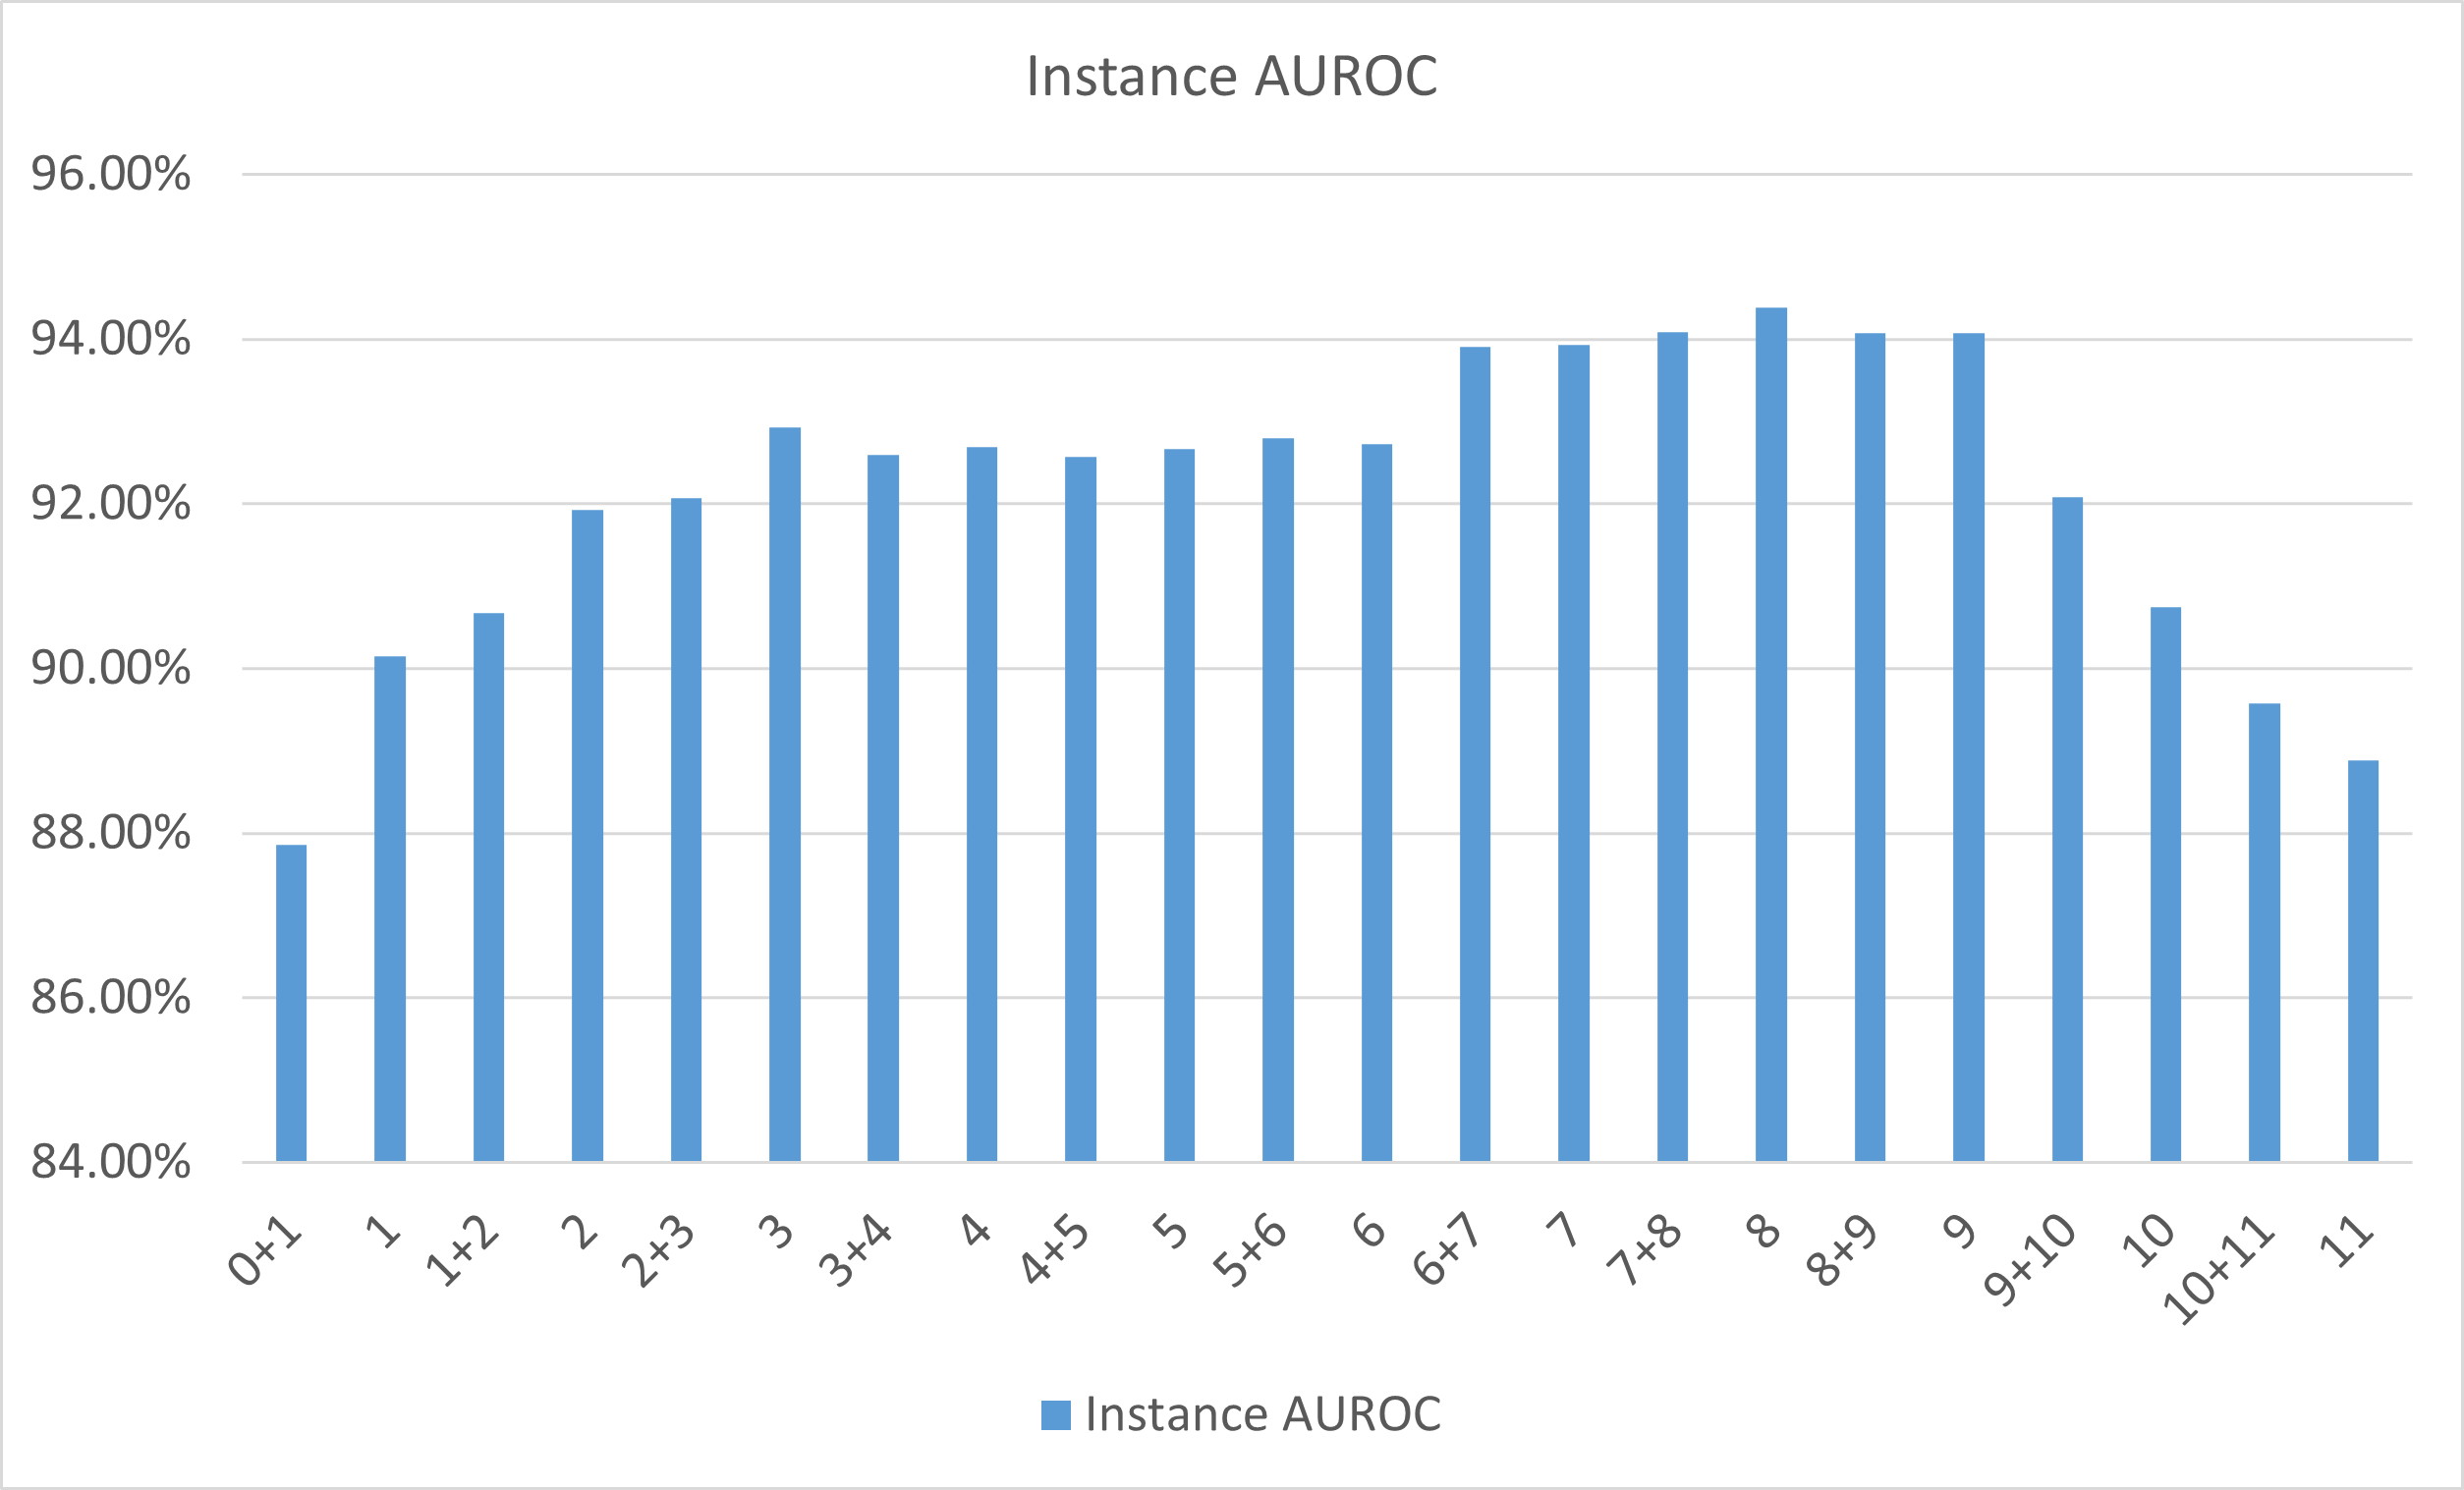
\includegraphics[width=1.0\linewidth]{Chapter_4/vit.png}
	\end{center}
	\caption{Medical Visual Question Answering (VQA) \cite{liu2021slake} is a task where the model receives medical images and corresponding questions as input and produces accurate answers as the output.}
	\label{fig:vit_layers}
\end{figure}